\documentclass[tikz,border=8pt]{standalone}
\usepackage{pgfplots}
\pgfplotsset{compat=1.18}
\definecolor{chapterteal}{HTML}{196F6B}
\definecolor{chaptergold}{HTML}{C58B18}

\begin{document}

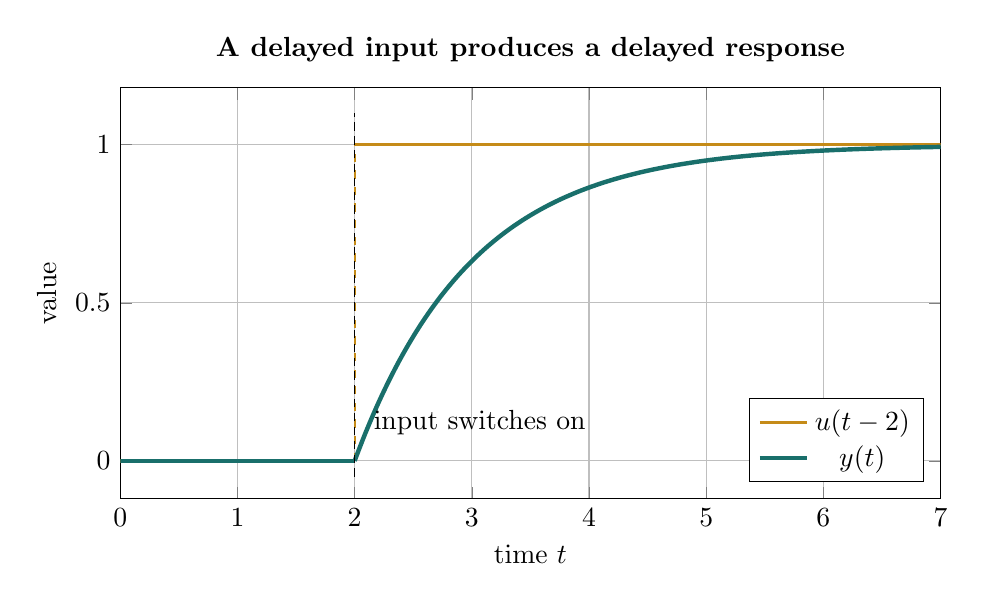
\begin{tikzpicture}
\begin{axis}[
  width=12cm,
  height=6.8cm,
  xmin=0,xmax=7,
  ymin=-0.12,ymax=1.18,
  xlabel={time $t$},
  ylabel={value},
  title={A delayed input produces a delayed response},
  title style={font=\bfseries},
  grid=both,
  xtick={0,1,2,3,4,5,6,7},
  ytick={0,0.5,1},
  legend style={at={(0.98,0.04)},anchor=south east}
]
\addplot[chaptergold,very thick] coordinates {(0,0) (2,0)};
\addplot[chaptergold,dashed,thick,forget plot] coordinates {(2,0) (2,1)};
\addplot[chaptergold,very thick,forget plot] coordinates {(2,1) (7,1)};
\addlegendentry{$u(t-2)$}
\addplot[chapterteal,ultra thick,domain=0:2,samples=2] {0};
\addplot[chapterteal,ultra thick,domain=2:7,samples=160,forget plot]
  {1-exp(-(x-2))};
\addlegendentry{$y(t)$}
\addplot[black,densely dashed,thin,forget plot] coordinates {(2,-0.05) (2,1.1)};
\node[anchor=south west] at (axis cs:2.08,0.05) {input switches on};
\end{axis}
\end{tikzpicture}

\end{document}
